\begin{subfigure}[t]{0.9\textwidth}
        \centering
        \begin{subfigure}[t]{0.19\textwidth}
            \centering
            \textrm{Frame 0} \medskip \\
            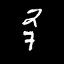
\includegraphics[scale=1]{figures/mnist0/frame0}
        \end{subfigure}
        \hfill
        \begin{subfigure}[t]{0.19\textwidth}
            \centering
            \textrm{Frame 4} \medskip \\
            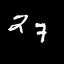
\includegraphics[scale=1]{figures/mnist0/frame4}
        \end{subfigure}
        \hfill
        \begin{subfigure}[t]{0.19\textwidth}
            \centering
            \textrm{Frame 8} \medskip \\
            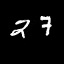
\includegraphics[scale=1]{figures/mnist0/frame8}
        \end{subfigure}
        \hfill
        \begin{subfigure}[t]{0.19\textwidth}
            \centering
            \textrm{Frame 12} \medskip \\
            
\includegraphics[scale=1]{figures/mnist0/frame12}
        \end{subfigure}
        \hfill
        \begin{subfigure}[t]{0.19\textwidth}
            \centering
            \textrm{Frame 16} \medskip \\
            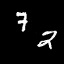
\includegraphics[scale=1]{figures/mnist0/frame16}
        \end{subfigure}
        \caption{Original Moving-MNIST frames.}
    \end{subfigure}
    \\ \bigskip
    \begin{subfigure}[t]{0.9\textwidth}
        \centering
        \begin{subfigure}[t]{0.19\textwidth}
            \centering
            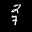
\includegraphics[scale=2]{figures/CKKS-DIFFERENCING/frame0}
        \end{subfigure}
        \hfill
        \begin{subfigure}[t]{0.19\textwidth}
            \centering
            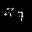
\includegraphics[scale=2]{figures/CKKS-DIFFERENCING/frame4}
        \end{subfigure}
        \hfill
        \begin{subfigure}[t]{0.19\textwidth}
            \centering
            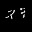
\includegraphics[scale=2]{figures/CKKS-DIFFERENCING/frame8}
        \end{subfigure}
        \hfill
        \begin{subfigure}[t]{0.19\textwidth}
            \centering
            
\includegraphics[scale=2]{figures/CKKS-DIFFERENCING/frame12}
        \end{subfigure}
        \hfill
        \begin{subfigure}[t]{0.19\textwidth}
            \centering
            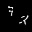
\includegraphics[scale=2]{figures/CKKS-DIFFERENCING/frame16}
        \end{subfigure}
        \caption{Frame Differencing with CKKS.}
    \end{subfigure}
    \\ \bigskip
    \begin{subfigure}[t]{0.9\textwidth}
        \centering
        \begin{subfigure}[t]{0.19\textwidth}
            \centering
            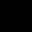
\includegraphics[scale=2]{figures/CKKS-MEAN/frame0}
        \end{subfigure}
        \hfill
        \begin{subfigure}[t]{0.19\textwidth}
            \centering
            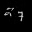
\includegraphics[scale=2]{figures/CKKS-MEAN/frame4}
        \end{subfigure}
        \hfill
        \begin{subfigure}[t]{0.19\textwidth}
            \centering
            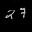
\includegraphics[scale=2]{figures/CKKS-MEAN/frame8}
        \end{subfigure}
        \hfill
        \begin{subfigure}[t]{0.19\textwidth}
            \centering
            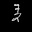
\includegraphics[scale=2]{figures/CKKS-MEAN/frame12}
        \end{subfigure}
        \hfill
        \begin{subfigure}[t]{0.19\textwidth}
            \centering
            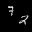
\includegraphics[scale=2]{figures/CKKS-MEAN/frame16}
        \end{subfigure}
        \caption{Mean Filter with CKKS.}
    \end{subfigure}
    \\ \bigskip
    \begin{subfigure}[t]{0.9\textwidth}
        \centering
        \begin{subfigure}[t]{0.19\textwidth}
            \centering
            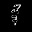
\includegraphics[scale=2]{figures/CKKS-GAUSSIAN/frame0}
        \end{subfigure}
        \hfill
        \begin{subfigure}[t]{0.19\textwidth}
            \centering
            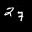
\includegraphics[scale=2]{figures/CKKS-GAUSSIAN/frame4}
        \end{subfigure}
        \hfill
        \begin{subfigure}[t]{0.19\textwidth}
            \centering
            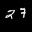
\includegraphics[scale=2]{figures/CKKS-GAUSSIAN/frame8}
        \end{subfigure}
        \hfill
        \begin{subfigure}[t]{0.19\textwidth}
            \centering
            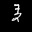
\includegraphics[scale=2]{figures/CKKS-GAUSSIAN/frame12}
        \end{subfigure}
        \hfill
        \begin{subfigure}[t]{0.19\textwidth}
            \centering
            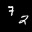
\includegraphics[scale=2]{figures/CKKS-GAUSSIAN/frame16}
        \end{subfigure}
        \caption{Gaussian Average with CKKS.}
    \end{subfigure}
    \\ \bigskip
    \begin{subfigure}[t]{0.9\textwidth}
        \centering
        \begin{subfigure}[t]{0.19\textwidth}
            \centering
            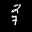
\includegraphics[scale=2]{figures/MeKKS-DIFFERENCING/frame0}
        \end{subfigure}
        \hfill
        \begin{subfigure}[t]{0.19\textwidth}
            \centering
            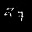
\includegraphics[scale=2]{figures/MeKKS-DIFFERENCING/frame4}
        \end{subfigure}
        \hfill
        \begin{subfigure}[t]{0.19\textwidth}
            \centering
            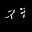
\includegraphics[scale=2]{figures/MeKKS-DIFFERENCING/frame8}
        \end{subfigure}
        \hfill
        \begin{subfigure}[t]{0.19\textwidth}
            \centering
            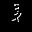
\includegraphics[scale=2]{figures/MeKKS-DIFFERENCING/frame12}
        \end{subfigure}
        \hfill
        \begin{subfigure}[t]{0.19\textwidth}
            \centering
            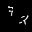
\includegraphics[scale=2]{figures/MeKKS-DIFFERENCING/frame16}
        \end{subfigure}
        \caption{Frame Differencing with MeKKS.}
    \end{subfigure}
    \\ \bigskip
    \begin{subfigure}[t]{0.9\textwidth}
        \centering
        \begin{subfigure}[t]{0.19\textwidth}
            \centering
            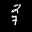
\includegraphics[scale=2]{figures/MeKKS-DIFFERENCING/frame0}
        \end{subfigure}
        \hfill
        \begin{subfigure}[t]{0.19\textwidth}
            \centering
            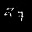
\includegraphics[scale=2]{figures/MeKKS-DIFFERENCING/frame4}
        \end{subfigure}
        \hfill
        \begin{subfigure}[t]{0.19\textwidth}
            \centering
            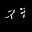
\includegraphics[scale=2]{figures/MeKKS-DIFFERENCING/frame8}
        \end{subfigure}
        \hfill
        \begin{subfigure}[t]{0.19\textwidth}
            \centering
            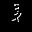
\includegraphics[scale=2]{figures/MeKKS-DIFFERENCING/frame12}
        \end{subfigure}
        \hfill
        \begin{subfigure}[t]{0.19\textwidth}
            \centering
            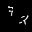
\includegraphics[scale=2]{figures/MeKKS-DIFFERENCING/frame16}
        \end{subfigure}
        \caption{Mean Filter with MeKKS.}
    \end{subfigure}
    \\ \bigskip
    \begin{subfigure}[t]{0.9\textwidth}
        \centering
        \begin{subfigure}[t]{0.19\textwidth}
            \centering
            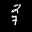
\includegraphics[scale=2]{figures/MeKKS-DIFFERENCING/frame0}
        \end{subfigure}
        \hfill
        \begin{subfigure}[t]{0.19\textwidth}
            \centering
            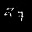
\includegraphics[scale=2]{figures/MeKKS-DIFFERENCING/frame4}
        \end{subfigure}
        \hfill
        \begin{subfigure}[t]{0.19\textwidth}
            \centering
            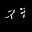
\includegraphics[scale=2]{figures/MeKKS-DIFFERENCING/frame8}
        \end{subfigure}
        \hfill
        \begin{subfigure}[t]{0.19\textwidth}
            \centering
            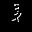
\includegraphics[scale=2]{figures/MeKKS-DIFFERENCING/frame12}
        \end{subfigure}
        \hfill
        \begin{subfigure}[t]{0.19\textwidth}
            \centering
            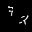
\includegraphics[scale=2]{figures/MeKKS-DIFFERENCING/frame16}
        \end{subfigure}
        \caption{Gaussian Average with MeKKS.}
    \end{subfigure}
